%%%%%%%%%%%%%%%%%%%%%%%%%%%%%%%%%%%%%%%%%%%%%%%%%%%%%%%%%%%%%%%%%%%%%%%%%%%%%%%%%
%% Documenclass 
%%%%%%%%%%%%%%%%%%%%%%%%%%%%%%%%%%%%%%%%%%%%%%%%%%%%%%%%%%%%%%%%%%%%%%%%%%%%%%%%%
\documentclass[a4paper,oneside,titlepage]{report}
%%%%%%%%%%%%%%%%%%%%%%%%%%%%%%%%%%%%%%%%%%%%%%%%%%%%%%%%%%%%%%%%%%%%%%%%%%%%%%%%%
%% Packages
%%%%%%%%%%%%%%%%%%%%%%%%%%%%%%%%%%%%%%%%%%%%%%%%%%%%%%%%%%%%%%%%%%%%%%%%%%%%%%%%%
\usepackage[english]{babel}
\usepackage{amsmath}
\usepackage{complexity}
\usepackage[T1]{fontenc}
\usepackage[utf8]{inputenc}
\usepackage[pdftex]{graphicx} %%Graphics in pdfLaTeX
\usepackage{a4wide} %%Smaller margins, more text per page.
\usepackage{longtable} %%For tables that exceed a page width
\usepackage{pdflscape} %%Adds PDF sup­port to the land­scape en­vi­ron­ment of pack­age
\usepackage{caption} %%Pro­vides many ways to cus­tomise the cap­tions in float­ing en­vi­ron­ments like fig­ure and ta­ble
\usepackage{float} %%Im­proves the in­ter­face for defin­ing float­ing ob­jects such as fig­ures and ta­bles
\usepackage[tablegrid,nochapter]{vhistory} %%Vhis­tory sim­pli­fies the cre­ation of a his­tory of ver­sions of a doc­u­ment
\usepackage[nottoc]{tocbibind} %%Au­to­mat­i­cally adds the bib­li­og­ra­phy and/or the in­dex and/or the con­tents, etc., to the Ta­ble of Con­tents list­ing
\usepackage[toc,page]{appendix} %%The ap­pendix pack­age pro­vides var­i­ous ways of for­mat­ting the ti­tles of ap­pen­dices
\usepackage{pdfpages} %%This pack­age sim­pli­fies the in­clu­sion of ex­ter­nal multi-page PDF doc­u­ments in LATEX doc­u­ments
\usepackage[rightcaption]{sidecap} %%De­fines en­vi­ron­ments called SC­fig­ure and SCtable (anal­o­gous to fig­ure and ta­ble) to type­set cap­tions side­ways
\usepackage{cite} %%The pack­age sup­ports com­pressed, sorted lists of nu­mer­i­cal ci­ta­tions, and also deals with var­i­ous punc­tu­a­tion and other is­sues of rep­re­sen­ta­tion, in­clud­ing com­pre­hen­sive man­age­ment of break points
\usepackage[]{acronym} %%This pack­age en­sures that all acronyms used in the text are spelled out in full at least once. It also pro­vides an en­vi­ron­ment to build a list of acronyms used
\usepackage[pdftex,scale={.8,.8}]{geometry} %%The pack­age pro­vides an easy and flex­i­ble user in­ter­face to cus­tomize page lay­out, im­ple­ment­ing auto-cen­ter­ing and auto-bal­anc­ing mech­a­nisms so that the users have only to give the least de­scrip­tion for the page lay­out. For ex­am­ple, if you want to set each mar­gin 2cm with­out header space, what you need is just \usep­a­ck­age[mar­gin=2cm,no­head]{ge­om­e­try}.
\usepackage{layout} %%The pack­age de­fines a com­mand \lay­out, which will show a sum­mary of the lay­out of the cur­rent doc­u­ment
\usepackage{subfigure} %%Pro­vides sup­port for the ma­nip­u­la­tion and ref­er­ence of small or ‘sub’ fig­ures and ta­bles within a sin­gle fig­ure or ta­ble en­vi­ron­ment.
\usepackage[toc]{glossaries} %%The glos­saries pack­age sup­ports acronyms and mul­ti­ple glos­saries, and has pro­vi­sion for op­er­a­tion in sev­eral lan­guages (us­ing the fa­cil­i­ties of ei­ther ba­bel or poly­glos­sia).
\usepackage[left,pagewise,modulo]{lineno} %%Adds line num­bers to se­lected para­graphs with ref­er­ence pos­si­ble through the LATEX \ref and \pageref cross ref­er­ence mech­a­nism
\usepackage[pdftex,colorlinks=false,hidelinks,pdfstartview=FitV]{hyperref}%%The hy­per­ref pack­age is used to han­dle cross-ref­er­enc­ing com­mands in LATEX to pro­duce hy­per­text links in the doc­u­ment. 
\usepackage{metainfo}
\usepackage[pagestyles,raggedright]{titlesec}
\usepackage{etoolbox}
\usepackage{%
	array, %%An ex­tended im­ple­men­ta­tion of the ar­ray and tab­u­lar en­vi­ron­ments which ex­tends the op­tions for col­umn for­mats, and pro­vides "pro­grammable" for­mat spec­i­fi­ca­tions
	booktabs, %%The pack­age en­hances the qual­ity of ta­bles in LATEX, pro­vid­ing ex­tra com­mands as well as be­hind-the-scenes op­ti­mi­sa­tion
	dcolumn, %%
	rotating,
	shortvrb,
	units,
	url,
	lastpage,
	longtable,
	lscape,
	qtree,
	skmath,	
}
%%%%%%%%%%%%%%%%%%%%%%%%%%%%%%%%%%%%%%%%%%%%%%%%%%%%%%%%%%%%%%%%%%%%%%%%%%%%%%%%%
%% Java --> latex 
%%%%%%%%%%%%%%%%%%%%%%%%%%%%%%%%%%%%%%%%%%%%%%%%%%%%%%%%%%%%%%%%%%%%%%%%%%%%%%%%%
\usepackage{listings}
\usepackage{color}
\definecolor{pblue}{rgb}{0.13,0.13,1}
\definecolor{pgreen}{rgb}{0,0.5,0}
\definecolor{pred}{rgb}{0.9,0,0}
\definecolor{pgrey}{rgb}{0.46,0.45,0.48}
\usepackage{inconsolata}
%%Listing style for java.
\definecolor{dkgreen}{rgb}{0,0.6,0}
\definecolor{gray}{rgb}{0.5,0.5,0.5}
\definecolor{mauve}{rgb}{0.58,0,0.82}
\lstset{frame=tb,
	language=Java,
	aboveskip=3mm,
	belowskip=3mm,
	showstringspaces=false,
	columns=flexible,
	basicstyle={\small\ttfamily},
	numbers=left,
	numberstyle=\tiny\color{gray},
	keywordstyle=\color{blue},
	commentstyle=\color{dkgreen},
	stringstyle=\color{mauve},
	breaklines=true,
	breakatwhitespace=true,
	tabsize=3
}

%%%%%%%%%%%%%%%%%%%%%%%%%%%%%%%%%%%%%%%%%%%%%%%%%%%%%%%%%%%%%%%%%%%%%%%%%%%%%%%%%
\setlength{\parindent}{0pt}
\setlength{\parskip}{.5\baselineskip}
%%%%%%%%%%%%%%%%%%%%%%%%%%%%%%%%%%%%%%%%%%%%%%%%%%%%%%%%%%%%%%%%%%%%%%%%%%%%%%%%%
%% Inserting the metadata
%%%%%%%%%%%%%%%%%%%%%%%%%%%%%%%%%%%%%%%%%%%%%%%%%%%%%%%%%%%%%%%%%%%%%%%%%%%%%%%%%
% % Metadaten des Dokumentes


\def\Institute{\textit{University of Nottingham}}
\def\Course{\textit{Computer Science}}
\def\Module{\textit{ Software Specification}}



\def\BoldTitle{Software Requirements Specification}

\def\Subtitle{for \\ Stress Relieving Game \\}
\def\Authors{Prepared by Vasilis Ieropoulos (4296039) } 
\def\Shortname{V.Ieropoulos}

\title{\textbf{\BoldTitle}\\\Subtitle}
\author{\Authors \\ \\ \\ \Institute\\ \Course\\ \Module\\ \Docent\\ \Assistant}
\date{13 May 2019}

%%%%%%%%%%%%%%%%%%%%%%%%%%%%%%%%%%%%%%%%%%%%%%%%%%%%%%%%%%%%%%%%%%%%%%%%%%%%%%%%%
%% Creation of pdf information
%%%%%%%%%%%%%%%%%%%%%%%%%%%%%%%%%%%%%%%%%%%%%%%%%%%%%%%%%%%%%%%%%%%%%%%%%%%%%%%%%
\hypersetup{pdfinfo={
		Title={Title},
		Author={TR},
		Subject={Report}
	}}
%%%%%%%%%%%%%%%%%%%%%%%%%%%%%%%%%%%%%%%%%%%%%%%%%%%%%%%%%%%%%%%%%%%%%%%%%%%%%%%%%
%% Creating the frontpage
%%%%%%%%%%%%%%%%%%%%%%%%%%%%%%%%%%%%%%%%%%%%%%%%%%%%%%%%%%%%%%%%%%%%%%%%%%%%%%%%%
\AtBeginDocument{
	\maketitle
	\thispagestyle{empty}
}

%%%%%%%%%%%%%%%%%%%%%%%%%%%%%%%%%%%%%%%%%%%%%%%%%%%%%%%%%%%%%%%%%%%%%%%%%%%%%%%%%
%% Creation of the header
%%%%%%%%%%%%%%%%%%%%%%%%%%%%%%%%%%%%%%%%%%%%%%%%%%%%%%%%%%%%%%%%%%%%%%%%%%%%%%%%%
\patchcmd{\chapter}{plain}{short}{}{} %$ <-- the header on chapter 1
%%%%%%%%%%%%%%%%%%%%%%%%%%%%%%%%%%%%%%%%%%%%%%%%%%%%%%%%%%%%%%%%%%%%%%%%%%%%%%%%%
%% Creation of page-styles
%%%%%%%%%%%%%%%%%%%%%%%%%%%%%%%%%%%%%%%%%%%%%%%%%%%%%%%%%%%%%%%%%%%%%%%%%%%%%%%%%
\newpagestyle{long}{%
	\sethead[\thepage][][\chaptername\ \thechapter:\ \chaptertitle]{\chaptername\ \thechapter:\ \chaptertitle}{}{\thepage}
	\headrule
}

\newpagestyle{short}{%
	\sethead[\thepage][][]{}{}{\thepage}
	\headrule
}
%%%%%%%%%%%%%%%%%%%%%%%%%%%%%%%%%%%%%%%%%%%%%%%%%%%%%%%%%%%%%%%%%%%%%%%%%%%%%%%%%
%% DOCUMENT
%%%%%%%%%%%%%%%%%%%%%%%%%%%%%%%%%%%%%%%%%%%%%%%%%%%%%%%%%%%%%%%%%%%%%%%%%%%%%%%%%
\begin{document}

\pagenumbering{roman}
\DeclareGraphicsExtensions{.pdf,.jpg,.png}
\pagestyle{short}



\newpage
%%%%%%%%%%%%%%%%%%%%%%%%%%%%%%%%%%%%%%%%%%%%%%%%%%%%%%%%%%%%%%%%%%%%%%%%%%%%%%%%%
%% Table of contents
%%%%%%%%%%%%%%%%%%%%%%%%%%%%%%%%%%%%%%%%%%%%%%%%%%%%%%%%%%%%%%%%%%%%%%%%%%%%%%%%%
 \tableofcontents % Inhaltsverzeichnis



\pagestyle{long}




%%%%%%%%%%%%%%%%%%%%%%%%%%%%%%%%%%%%%%%%%%%%%%%%%%%%%%%%%%%%%%%%%%%%%%%%%%%%%%%%%
%% Version table insertion
%%%%%%%%%%%%%%%%%%%%%%%%%%%%%%%%%%%%%%%%%%%%%%%%%%%%%%%%%%%%%%%%%%%%%%%%%%%%%%%%%
% Versionstabelle.

\chapter*{Revision History}
\addcontentsline{toc}{chapter}{Revision History}
\begin{versionhistory}
	\vhEntry{1.0}{29.03.2019}{V.Ieropoulos}{Chapter 1 - Introduction}
    \vhEntry{2.0}{08.04.2019}{V.Ieropoulos}{Chapter 2 - Overall Description}
    \vhEntry{3.0}{15.04.2019}{V.Ieropoulos}{Chapter 3 - External Interface Requirements}
    \vhEntry{4.0}{29.04.2019}{V.Ieropoulos}{Chapter 4 - System Features}
    \vhEntry{5.0}{08.05.2019}{V.Ieropoulos}{Chapter 5 - Other Nonfunctional Requirements}

\end{versionhistory}
\pagenumbering{arabic}
%%%%%%%%%%%%%%%%%%%%%%%%%%%%%%%%%%%%%%%%%%%%%%%%%%%%%%%%%%%%%%%%%%%%%%%%%%%%%%%%%
%% Inserting all the content
%%%%%%%%%%%%%%%%%%%%%%%%%%%%%%%%%%%%%%%%%%%%%%%%%%%%%%%%%%%%%%%%%%%%%%%%%%%%%%%%%
\chapter{Introduction}
\label{ch:intro}

\section{Purpose}
This Software Requirements Specification(SRS) document is intended to give a complete overview of the game Adventures of V man(AVM). The SRS document details all the features upon which AVM has currently decided to implement.  
\section{Document Conventions}
This document makes use of the following acronyms and it is advised for the reader to reference back to the table for any clarification. 

\begin{center}
 \begin{tabular}{||c c||} 
 \hline
 Acronym & Meaning \\ [0.5ex] 
 \hline\hline
 SRS & Software Requirements Specification \\ 
 \hline
 AVM & Adventures of V man  \\
 \hline
\end{tabular}
\end{center}




\section{Intended Audience and Reading Suggestions}
The Adventures of V man is a prototype for the stress reducing game.This has been implemented under the guidance of University professors. This project is useful for people trying to reduce stress as well as to the average gamer wanting to play a casual game.


\section{Product Scope}
The Adventures of V man is a simple platforming shooter game that call upon the player to shoot up oncoming enemies until they reach the end of the level where they are faced with the a big boss battle.
The game is minimal in design so that it can be run on almost any device.The main character of the game is controlled by using the arrow keys on the keyboard, uses the space bar to jump and also uses the "Z" button to fire at enemies with balls of fire.
The Adventures of V man must help the player in reducing his stress there for a straight forward and easy to understand game is required so that not much thought is put into playing the game. The program is based on a mix of 8bit and 16bit characters and animations giving a sense of nostalgia to the player.

\section{References}
 Brakeys: \href{https://github.com/Brackeys/2D-Character-Controller}{Character Controller physics}


\chapter{Overall Description}
\label{Overall Description}

\section{Product Perspective}
\paragraph{}The game itself is not derived from an other game it is being implemented with the development tool Unity which gives us the ability to compile it on platforms such as Windows , Linux and MacOS. In addition it also gives us the ability to port it as an android application.

\paragraph{}The game is focused on game play and does not focus on any particular story line since this is a stress reducing game having a story line would make no difference since the user would want to play a game straight away without the hassle of going through lines and lines text explaining the story.

\paragraph{} The game must have these features:
\begin{itemize}
    \item Colourful and cheer full so that the user can have a sense of happiness 
    \item Easy to play to game such that no instructions are needed 
    \item Responsive and easy to control  
\end{itemize}
\section{Game Functions}
The following is a summary of major functions implemented in the game.
\subsection{Functions}
\begin{itemize}
    \item Jumping
    A necessary mechanic of the game which allow sudden movements when trying to avoid enemies , cross obstacles or attack enemies which are higher up.
    \item Attack
    The fundamental mechanic to beating the game as it requires the player to kill enemies to reach the end boss. The attack mechanic fires "balls of fire" which deal damage to enemies.
    \item Crouch
    The player can crouch so he can get through tight places it also slows the player down which can help in moving more precisely.
\end{itemize}
\section{User Classes and Characteristics}
The game controls are designed to be simple and intuitive.Players at any age level should be able to pick up the game and play without any instructions.The game implements one difficulty level so it can be equal to every one. 
What will distinguish players from each other is : 
\begin{itemize}
    \item \textbf{Speed} The ability to beat the game as fast as possible
    \item \textbf{Foresight} The ability to plan out the paths of multiple enemies attacking the player and creating a strategy to to beat them in the most optimal and efficient way.
    \item \textbf{Intuition} The ability to make a calculated guess of the position of off-screen objects.
    
\end{itemize}

\subsection{User story}
Matt is very stressed out due to exams and needs something to relieve that stress, so he Downloads and installs a game to help him get away from all that stress.He requires a game that is easy , small and simple so that he doesn't have to do much thinking.

\subsection{Use Case Diagram}
\begin{figure}[hbt!]
    \centering
    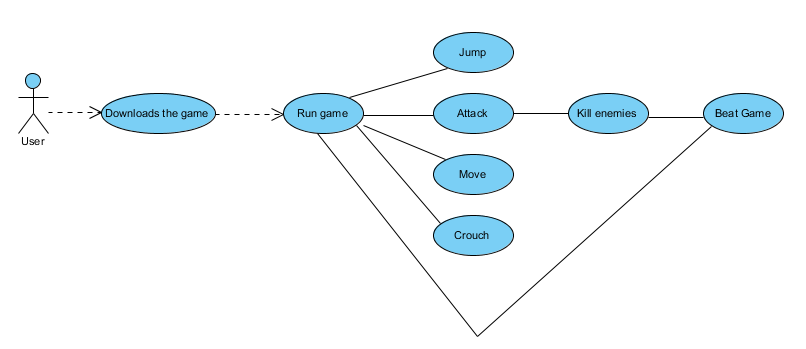
\includegraphics[width=100mm,scale=0.6]{images/diagram.png}
    \caption{Use Case Diagram}
    \label{fig:diagram}
\end{figure}
\section{Operating Environment}

Operating environment for AVM  is as listed below.
\begin{itemize}
    \item \textbf{Operating System}: Windows , Linux , Mac-OS
    \item \textbf{Platform}: Unity 2D
\end{itemize}

\section{Design and Implementation Constraints}
\subsection {Design}
The design of the game is based on 8 and 16 bit characters and sprites that bring back nostalgic feelings to the user. The layout is cheerful and straightforward.The colours used are bright and vivid to induce a sense of happiness the user.Since this game is for stress reduction this is appropriate.
\subsection{Implementation}
The game is implemented in Unity. Every thing is made from scratch including sprites,sounds and layout.
The sprites where made using online 8bit paint programs like \href{https://www.piskelapp.com/}{PiskelApp}.
The sounds where made using \href{https://www.image-line.com/flstudio/}{FL-Studio} and a \href{https://www.amazon.co.uk/AKAI-Professional-LPK25-Portable-Controller/dp/B002M8GBDI}{AKAI LPK25} which is a midi keyboard.
We could have used other software to create the sounds and the keyboard was not necessary but it did make things easier.
\section{Tools}
\begin{itemize}
	\item \textbf{Programming Language :} C\#
	\item \textbf{Programming IDE :} Notepad ++
	\item \textbf{Programming Framework :} Unity2d
	\item \textbf{Report Writing :} Overleaf/Latex
\end{itemize}
\newpage




\chapter{External Interface Requirements}
\label{External Interface Requirements}

\section{User Interfaces}

\begin{itemize}
    \item \textbf{Front-End Software:} Unity 2D
    \item \textbf{Back-End Software:} C \#
\end{itemize}

\section{Hardware Interfaces}
\begin{itemize}
    \item Windows / Linux / Mac Os
\end{itemize}

\section{Software Interfaces}
The following is the software used for AVM :

\begin{center}

 \begin{tabular}{ l p {10cm}}
 
 \hline
 Software used & Description \\ [0.5ex] 
 \hline\hline
 Operating System & we have chosen to make the game cross platform to cater to all users but have written the game on windows since unity is not officially supported on Linux \\ 
 \hline
 Unity & We have chosen Unity as its a free cross platform framework that works on a plethora of Operating systems  \\
 \hline
 
\end{tabular}

\end{center}




\section{Communications Interfaces}
Players of the game wont need to install any additional software packages such as Direct X. Unity relies only on packages which as pre-installed on most operating systems.

\chapter{System Features}
\label{System Features}

\section{Jumping}
\subsection{Description and Priority}
Being one of the most important game mechanic in any game it allows the player to navigate gaps and dodge enemy attacks.Also it help the player attack enemies that might be jumping as well.
\subsection{Stimulus}
\begin{itemize}
    \item \textbf{Step 1:} The player presses the space button to jump
    \item \textbf{Step 2:} The character jumps upwards with a constant force.
\end{itemize}
\subsection{Functional Requirements:}
\begin{itemize}
    \item \textbf{Requirements 1:} Because the player can only jump once before he touches the ground there must be a standardized amount of force the player can jump.
    \item \textbf{Requirements 2:} There should be different variations to the level to allow the player to jump.
\end{itemize}

\section{Attacking}
\subsection{Description and Priority}
This is fundamental to the game itself as the game requires the player to kill enemies so they can progress to the final boss and ultimately finish the game.
\subsection{Stimulus}
\begin{itemize}
    \item \textbf{Step 1:} The player presses the Z button to fire
    \item \textbf{Step 2:} The character fires a projectile the deals damage when it hits an enemy and destroys it self afterwards.
\end{itemize}
\subsection{Functional Requirements:}
\begin{itemize}
    \item \textbf{Requirements 1:} The damage the attack deals needs to be constant.
    \item \textbf{Requirements 2:} Different enemies should have different amounts of health.
\end{itemize}

\section{Crouching}
\subsection{Description and Priority}
This is a mechanic in the game that can be used not only to navigate the map but also dodge incoming attacks. This lowered the height of the player and slows him down.
\subsection{Stimulus}
\begin{itemize}
    \item \textbf{Step 1:} The player presses the Down arrow to crouch.
    \item \textbf{Step 2:} The character can then move around slower and move under tight spots. 
\end{itemize}
\subsection{Functional Requirements:}
\begin{itemize}
    \item \textbf{Requirements 1:} The player cant jump while crouching.
    \item \textbf{Requirements 2:} The player can move backwards while crouching.
\end{itemize}
\chapter{Other Nonfunctional Requirements}
\label{Other Nonfunctional Requirements}

\section{Performance Requirements}
Based on the capabilities of current computers and the state of Windows/Linux/MacOs performance of the game should not be an issue since its a very small game prototype that uses minimal resources.However some systems that wont be able to not run unity correctly might have some performance issues. The game design will be tailored for use on the most basic computer system for an enjoyable experience for everyone.The game will be overly simplistic and trivial as well as the graphics will not be detailed so that they do not take up a lot of system resources. 
\section{Safety Requirements}
AVM will not affect any other part of the operating system other than the parts needed to run the game.The game must not be played by the player when they are dividing their attention to multiple tasks since this is meant to be a stress reducing game. Hence to reduce stress the player must only focus on the game and not anything else to prevent potential harm to the player.
\section{Security Requirements}
AVM will not ask for any personal information from the player and therefor will be unable to compromise such information.There is no high score or  player authentication so no data is being recorded. The player thus only need to download and play the game in order to start playing.That said if anyone has access to the players computer they inherently have access to his data which is beyond the scope of the game and our responsibility.
\section{Software Quality Attributes}
To ensure the game is reliable , AVM will respond instantly to the users commands. When the player makes the character jump the gravity and velocity components of the game will respond immediately, the player should see the effect of his actions in milliseconds not a few seconds after. This way we can limit the amount of stress the player will endure and alternatively help in reducing the stress.
In terms of usability, the overall game will be straightforward so that the player wont need any explaining to on how to play.Since there is only one level in the game there is no need to increase the difficulty gradually but we can keep a constant level of difficulty throughout the level.It should be a game that any player can instantly pick up and play without having much time to figure out the controls.The controls will be easy and intuitive to use and the player will not be bombarded by having to use all the controls at once.





%%%%%%%%%%%%%%%%%%%%%%%%%%%%%%%%%%%%%%%%%%%%%%%%%%%%%%%%%%%%%%%%%%%%%%%%%%%%%%%%%
%% Source defintions
%%%%%%%%%%%%%%%%%%%%%%%%%%%%%%%%%%%%%%%%%%%%%%%%%%%%%%%%%%%%%%%%%%%%%%%%%%%%%%%%%
% When no use outcomment
%\bibliographystyle{alpha}

\renewcommand\bibname{References}
\bibliography{base/sources}


%%%%%%%%%%%%%%%%%%%%%%%%%%%%%%%%%%%%%%%%%%%%%%%%%%%%%%%%%%%%%%%%%%%%%%%%%%%%%%%%%
%% Inserting the appendix
%%%%%%%%%%%%%%%%%%%%%%%%%%%%%%%%%%%%%%%%%%%%%%%%%%%%%%%%%%%%%%%%%%%%%%%%%%%%%%%%%
% When no use outcomment
%\newpage
\appendix 
% Adds appendix as chapter to toc
\addcontentsline{toc}{chapter}{Appendix}


\chapter{First}


\chapter{Second}


\end{document}*/***********************************************************************8	
